La mayor\'ia de las actividades que una persona realiza son en grupo \cite{ellis1991groupware}, para el apoyo a este tipo de actividades existen los sistemas groupware que son aquellos que apoyan a personas ocupadas en una tarea en com\'un, y que proveen una interfaz a un ambiente compartido, \cite{ellis1991groupware} cuyo objetivo es facilitar la comunicaci\'on, cooperaci\'on, y coordinaci\'on de los usuarios, seg\'un Cruz \cite{cruz2012towards} la comunicaci\'on se entiende como el proceso de interacci\'on entre personas que incluye el intercambio impl\'icito o expl\'icito de informaci\'on; Malone \& Crowston \cite{malone1994interdisciplinary} definieron coordinaci\'on como el manejo de interdependencias entre actividades realizadas por multiples actores basadas en objetos mutuos que son intercambiados entre actividades; la cooperaci\'on ocurre cuando un grupo trabaja para lograr una misma meta \cite{malone1994interdisciplinary} con alto grado de tareas interdependientes, compartiendo la informaci\'on disponible a trav\'es de alguna clase de espacio compartido. Existen diferentes tipos de sistemas groupware, \cite{ellis1991groupware} define 2 clasificaciones: por espacio-tiempo y por tipo de aplicaci\'on. Entre el rubro espacio-tiempo se encuentran aquellos que su funcionalidad permite interacciones cara a cara o interacciones distribuidas, as\'i mismo podemos encontrar aquellos que permiten una interacci\'on en tiempo real o una interacci\'on as\'incrona. Adem\'as de s\'incronos y as\'incronos agrega un tercer rubro que es la mixta que combina los dos anteriores, y engloba todos en la caracter\'istica de tipo de comunicaci\'on, y para la interacci\'on de los usuarios agrega la caracter\'istica de saber si el usuario est\'a conectado o desconectado en caso de las interacciones distribuidas, estas las incluye en la categor\'ia de disponibilidad del usuario\cite{antunes2014reviewing}.

Por otra parte cuando se toma en cuenta el tipo de aplicaci\'on para clasificar los sistemas groupware, podemos encontrar los siguientes: Sistemas de mensajes que soportan el intercambio as\'incrono de mensajes entre miembros de un grupo; editores multiusuario que permite a miembros de un grupo crear y editar un mismo documento al mismo tiempo, pueden ser s\'incronos o as\'incronos; sistemas para soporte de decisiones de grupo y cuartos electr\'onicos de reuniones, proveen infraestructura para la exploraci\'on de problemas no estructurados en un grupo; c\'omputo para conferencias: proporciona servicios como medios de comunicaci\'on en muchas formas, hay 3 tipos: de tiempo real, teleconferencia, y de escritorio; y por \'ultimo los agentes inteligentes que son programas computacionales \textit{inteligentes} encargados de tareas espec\'ificas.

Adem\'as de esta clasificaci\'on Ellis\cite{ellis1991groupware} propone elementos que tienen que ser tomados en cuenta para poder comparar y describir a los sistemas groupware, entre ellos se encuentran el contexto compartido que es el ambiente en el que va a correr el sistema; un grupo de ventanas que son las que se van a mostrar en diferentes pantallas del sistema y se van a compartir; un tele apuntador que es la capacidad de m\'as de un usuario de mover el apuntador al mismo tiempo; vista, es la porci\'on de contexto o ambiente que se va a mostrar en diferentes ventanas del sistema; sesi\'on que son los tipos de interacci\'on del usuario con el sistema y que ya se mencionaron antes (mismo tiempo, mismo lugar; diferente tiempo, diferente lugar, etc.) y los roles que son los tipos de usuarios que hay y los derechos y permisos que tienen con el sistema.

Shmidt \cite{schmidt1992taking} menciona varias propiedades que deben de tener los sistemas groupware:
\begin{itemize}
\item Es social; objeto, sujeto, medios, fines, motivos y necesidades, competencias e implementaciones, est\'an mediadas socialmente.
\item Integrantes mutuamente dependientes, necesitan cooperar para terminar el trabajo. Diferente a solo compartir el mismo recurso, sujeto A conf\'ia positivamente en la calidad y l\'ineas de tiempo del trabajo de sujeto B y vice versa
\item Distribuci\'on de tareas qu\'e va a hacer cada individuo, cu\'ando y d\'onde.
\item Distribuci\'on f\'isica en tiempo y espacio
\item Distribuci\'on l\'ogica, en t\'erminos de control, en el sentido de que los sistemas son semi aut\'onomos en su trabajo parcial.
\item Deben aumentar las capacidades mec\'anicas y de procesamiento de informaci\'on del individuo.
\item Deben combinar las actividades especializadas de m\'ultiples trabajadores dedicados a las diferentes herramientas especializadas.
\item Deben facilitar las aplicaciones de m\'ultiples problemas resolviendo estrategias y heur\'isticas de un problema dado.
\item Deben facilitar la aplicaci\'on de m\'ultiples perspectivas y concepciones de un problema dado para adaptarse a naturaleza m\'ultiple del ambiente de trabajo.
\item Deben apoyar la auto organizaci\'on, de conjuntos cooperativos al contrario de interrumpir trabajo cooperativo computarizando procedimientos formales.
\end{itemize}

Para Shmidt \cite{schmidt1992taking} el trabajo colaborativo es siempre social, en el sentido en el que el objeto y el sujeto, los fines y los medios, los motivos y necesidades est\'an mediados socialmente, cada elemento del grupo depende, en parte, del trabajo de alg\'un otro miembro y viceversa, y cuando esto sucede, es importante que ambos elementos del grupo tengan el conocimiento de los avances del otro para poder hacer una estimaci\'on de sus propias acciones, esto es, que cada miembro tenga conciencia de lo que pasa a su alrededor para que pueda tomar demisiones adecuadas en cuanto a la actividad que tiene asignada en el grupo.

\section{Consciencia}

Gutwin \cite{gutwin1996supporting} menciona que es importante que los individuos sepan lo que est\'an haciendo los dem\'as ya que pueden usar ese conocimiento para anticipar las acciones de los otros, y ayudarlos con sus tareas, Dourish y Bellotti \cite{dourish1992awareness} fueron los primeros en introducir el t\'ermino awareness diciendo que es el entendimiento de las actividades de otros, que proporciona un contexto para tu propia actividad, a\'un m\'as, dicen que este contexto es usado para asegurar que las contribuciones individuales sean relevantes a las actividades del grupo como un todo, y para evaluar las acciones individuales con respecto a los objetivos del grupo y progresos. 

En un estudio realizado por \cite{Belkadi2013110} se mencionan las caracter\'isticas que debe de tener la consciencia o el conocimiento, entre ellas se encuentran el tener muchas facetas, es decir, existen diferentes tipos de conocimiento como se explicar\'a m\'as adelante; el conocimiento est\'a fuertemente enlazado a situaciones colaborativas ya que los colaboradores necesitan informaci\'on para llevar a cabo algunas tareas o para tomar decisiones; el conocimiento en una situaci\'on colaborativa puede incrementar los niveles de confianza entre actores lo que los alienta a compartir informaci\'on. Adem\'as de estas caracter\'isticas proponen 3 tipos de conocimiento, o consciencia: Consciencia social, Consciencia de las tareas y Consciencia del espacio de trabajo; estas tres categor\'ias se pueden identificar con las preguntas de la siguiente tabla:

\begin{center}
\begin{longtable}{|p{2cm}|p{11cm}|}
\caption{Preguntas para entender los tipos de consciencia.}\\
\hline
\textbf{Tipo de consciencia} & \textbf{Preguntas}\\
\hline
\endfirsthead
\multicolumn{2}{c}%
{\tablename\ \thetable\ -- \textit{Contin\'ua de p\'agina anterior}} \\
\hline
\textbf{Tipo de consciencia} & \textbf{Preguntas} \\
\hline
\endhead
\hline \multicolumn{2}{r}{\textit{Contin\'ua en siguiente p\'agina}} \\
\endfoot
\hline
\endlastfoot

	Consciencia Social & ?`Qu\'e debo de esperar de otros miembros del grupo? ?`C\'omo voy a interactuar con el grupo? ?`Qu\'e rol voy a tomar en este grupo? ?`Qu\'e roles van a tomar los dem\'as miembros del grupo? \tabularnewline \hline
	Consciencia de las Tareas & ?`Qu\'e s\'e de este tema y la estructura de la tarea? ?`Qu\'e saben los dem\'as? ?`Qu\'e se necesita para completar la tarea? ?`C\'omo ser\'an evaluados los resultados? ?`Qu\'e herramientas u objetos se necesitan para completar esta tarea? ?`Cu\'anto tiempo se necesita y cu\'anto tiempo hay disponible? \tabularnewline \hline	
	Consciencia del espacio de trabajo & ?`Qu\'e hacen los dem\'as miembros del grupo para completar la tarea? ?`D\'onde est\'an? ?`Est\'an activos en el espacio de trabajo? ?`Qu\'e har\'an? ?`Qu\'e hacen actualmente? ?`Qu\'e han hecho? ?`Qu\'e har\'an despu\'es? ?`C\'omo los puedo ayudar? \tabularnewline
	\hline
\end{longtable}
\end{center}

Por otro lado  \cite{antunes2014reviewing} identifica seis tipos diferentes de consciencia; la consciencia colaborativa, la consciencia contextual, consciencia social, consciencia del espacio de trabajo, consciencia situacional, y consciencia del lugar.

\subsection{Consciencia colaborativa}

Ha sido generalmente aceptado como la percepci\'on de la disponibilidad del grupo que tiene cada uno de los integrantes. Disponibilidad del grupo quiere decir el conocimiento de si las personas est\'an en el mismo lugar f\'isico, o si est\'an conectados o desconectados y los medios de comunicaci\'on que tienen disponibles para colaborar entre s\'i.

\subsection{Conciencia contextual}

La conciencia contextual es fundamental para permitir que un grupo colaborativo tenga conocimiento de lo que est\'a pasando en el espacio virtual del sistema.

\subsection{Conciencia social}

La conciencia social \cite{antunes2014reviewing} apunta la importancia de entender las pr\'acticas sociales, como los roles de otros y sus actividades, o c\'omo est\'an otros miembros del grupo contribuyendo a una tarea.

\subsection{Conciencia de espacio de trabajo}

La conciencia del espacio de trabajo se divide en 2 aspectos: uno se enfoca en el lugar y el otro se enfoca en el espacio, otra cosa importante a considerar es la interacci\'on del grupo con los lugares de trabajo, finalmente la noci\'on del espacio de trabajo trae consigo el nivel de interdependencia de una tarea realizada por el grupo, considerando soporte de actividades paralelas, actividades coordinadas y actividades mutuamente ajustadas.

\subsection{Conciencia situacional}

Est\'a caracterizado por tres niveles cognitivos: en el primero una percepci\'on global del ambiente construido por eventos, acciones, recursos y otros elementos, en el segundo nivel se le da un sentido a lo que est\'a pasando actualmente y en el tercero se construyen escenarios a futuro.

\subsection{Conciencia del lugar}

Puede referirse al conocimiento de los elementos de una ubicaci\'on geogr\'afica como pueden ser coordenadas, orientaci\'on, distancia, etc. O tambi\'en el conocimiento de los elementos de un espacio f\'isico, incluyendo clima, topolog\'ia f\'isica del lugar, y atributos f\'isicos.

\newpage
\section*{}


Por la naturaleza de los sistemas groupware las \'areas de m\'as inter\'es son la conciencia social y la conciencia del espacio de trabajo. En otra clasificaci\'on (Gutwin, C., Greenberg, S., \& Roseman, M., 1996) podemos encontrar 2 tipos de conciencia al contexto: primero conciencia general de las personas en una comunidad de trabajo, y segundo conciencia de las interacciones de otros en un espacio compartido.

Gutwin (Gutwin, Carl, Greenberg, Saul 1996) propone un marco de trabajo que considera elementos que incluyen mecanismos para recolectar informaci\'on \'util para la conciencia de la situaci\'on por parte de las personas, y que integran el conocimiento consciente del espacio de trabajo de un grupo.

\begin{center}
\begin{longtable}{|l|p{8cm}|}
\caption{Elementos de conciencia de la situaci\'on propuestos por Gutwin\cite{gutwin1996supporting}}\\
\hline
\textbf{Elementos} & \textbf{Cuestiones que responden}\\
\hline
\endfirsthead
\multicolumn{2}{c}%
{\tablename\ \thetable\ -- \textit{Contin\'ua de p\'agina anterior}} \\
\hline
\textbf{Elementos} & \textbf{Cuestiones que responden} \\
\hline
\endhead
\hline \multicolumn{2}{r}{\textit{Contin\'ua en siguiente p\'agina}} \\
\endfoot
\hline
\endlastfoot

Presencia & ?`Qui\'enes est\'an participando en la actividad?\\
Ubicaci\'on & ?`D\'onde est\'an trabajando?\\
Nivel de actividad & ?`Qu\'e tan activos son en el espacio de trabajo?\\
Acciones & ?`Cu\'ales son sus actividades y tareas actuales?\\
Intenciones & ?`Qu\'e har\'an despu\'es?, ?`D\'onde van a estar?\\
Cambios & ?`Qu\'e cambios est\'an realizando y en d\'onde?\\
Objetos & ?`Qu\'e objetos est\'an usando?\\
Extensiones & ?`Qu\'e pueden ver?, ?`Cu\'ales son sus alcances?\\
Habilidades & ?`Qu\'e pueden hacer?\\
Esfera de influencia & ?`D\'onde pueden hacer cambios?\\
Expectativas & ?`Qu\' se necesita que haga ahora?\\
\hline
\end{longtable}
\label{elem:context}
\end{center}

Todos los elementos de la tabla \ref*{elem:context} se pueden clasificar en dos grupos: aquellos que se encargan de saber que est\'a pasando con otras personas, y aquellos que se encargan de saber d\'onde est\'a pasando. Esta clasificaci\'on detalla el perfil individual de cada integrante y sigue las actividades de cada uno. En otro caso, en el trabajo de Montan\'e \cite{montane2013context} se propone un modelo de contexto social, donde hay categor\'ias similares, pero tomando en cuenta las relaciones entre los sujetos adem\'as de las actividades y estado actual de cada uno de ellos, los elementos que lista en su trabajo est\'an divididos en tres categor\'ias. La interactiva describe a los usuarios de forma individual y sus interacciones con las cosas que los rodean como objetos, tareas, eventos, usuarios o ubicaciones; la cohesiva integra elementos que tienen que ver con la actividad grupal y se pueden encontrar los grupos, roles, metas, alianzas, actividades y reglas. Y las afectivas que describe c\'omo se sienten los miembros del grupo al realizar las actividades entre ellas est\'an los sentimientos y los gestos.

\section{Consciencia del contexto}
Todos los elementos antes mencionados hacen referencia a la conciencia de parte del usuario del contexto que lo rodea, pero ?´es posible hacer que la conciencia del ambiente pueda ser aprendida por el propio sistema groupware? Existen sistemas groupware que son capaces de reconocer aspectos contextuales que rodean a un grupo de usuarios, estos sistemas son llamados conscientes del contexto, la informaci\'on contextual m\'as com\'un en los sistemas groupware es la ubicaci\'on f\'isica del usuario. Al hablar de sistemas groupware conscientes del contexto surgen algunos asuntos importantes que estos han de tomar en cuenta. Para empezar hace falta una categorizaci\'on formal del contexto en el que van a trabajar, el problema de esto es que los sistemas son desarrollados para que funcionen en \'ambitos espec\'ificos al problema o situaci\'on a la que se le quiere dar soluci\'on.

El conocimiento contextual describe una situaci\'on, la forma en la que se usan los elementos en un grupo de trabajo, incluyendo los eventos que son manejados por el grupo \cite{brezillon2004context}. Varios autores tienen un concepto de contexto algunos de ellos traslapan en definici\'on con otros, y diferentes elementos son tomados en cuenta para la descripci\'on de contexto. Dey \cite{dey2001conceptual} toma varias definiciones de contexto que otros autores hab\'ian hecho antes y hace su definici\'on que est\'a enfocada en el contexto en la computaci\'on, dice que contexto como cualquier tipo de informaci\'on que se puede usar para caracterizar la situaci\'on de entidades (se entiende por entidad una persona, lugar u objeto) que es considerada relevante para la interacci\'on entre un usuario y una aplicaci\'on incluyendo al usuario y la aplicaci\'on mismos.

Malik \cite{malik2007future} hace referencia a varios problemas que hay en la actualidad inherentes a consciencia contextual, entre ellos est\'an la definici\'on del contexto, ya que contexto es un concepto que abarca todos los posibles par\'ametros que identifican una situaci\'on, las aplicaciones y marcos de trabajo est\'an limitados a definir los par\'ametros del contexto de su propio \'ambito. Otro problema importante es que las arquitecturas no est\'an demasiado desarrolladas aun, est\'an desarrolladas para tareas espec\'ificas, hace falta est\'andares para definir una arquitectura y herramientas, por \'ultimo otro problema que es de inter\'es para este trabajo es la interpretaci\'on del contexto y las adaptaciones del comportamiento del servicio. 

Br\'ezillon \cite{brezillon2004context} estudia 3 casos de sistemas groupware conscientes al contexto y describe la forma en que apoya a la conciencia del contexto con los usuarios. SisPro es un sistema que tiene por objetivo facilitar las actividades colaborativas y procesos de aprendizaje y el desarrollo de competencias de trabajo colaborativo. SISCO tiene como tarea la preparaci\'on de reuniones,  da a conocer a los usuarios los temas de los que se est\'a hablando basados en su agenda individual. CO2DE es un software que permite unir los contextos individuales en un solo diagrama proporcionando una infraestructura de edici\'on colaborativa. Otro caso de sistema groupware muy diferente a los anteriores es Assault Cube \cite{montane2013context}, un juego FPS (Fisrt Shoter Person) de c\'odigo abierto que soporta las actividades colaborativas, en este varios jugadores se conectan a un servidor para llevar a cabo actividades espec\'ificas de la modalidad del juego que hayan escojido, el juego ofrece mecanismos de conciencia a los jugadores tales como un mapa de la ubicaci\'on del enemigo, un medidor de vitalidad, una pantalla de mensajes para comunicar al equipo, etc.

En figura 1 Se realiza una comparaci\'on tomando en cuenta los sistemas anteriores, para poder realizar las comparaciones se listan algunos aspectos propuestos por Gutwin \cite{gutwin1996supporting}, Montan\'e \cite{montane2013context}, Dey \cite{dey2001conceptual} y se clasifican en rubros m\'as grandes propuestos por Dey en otro de sus trabajos que son ambiente de usuario y ambiente f\'isico, el ambiente computacional, aunque es introducido por Dey, no es tomado en cuenta en ninguno de los sistemas ni en otras clasificaciones, as\'i que es omitido.

\begin{figure}[h!]
  \centering
    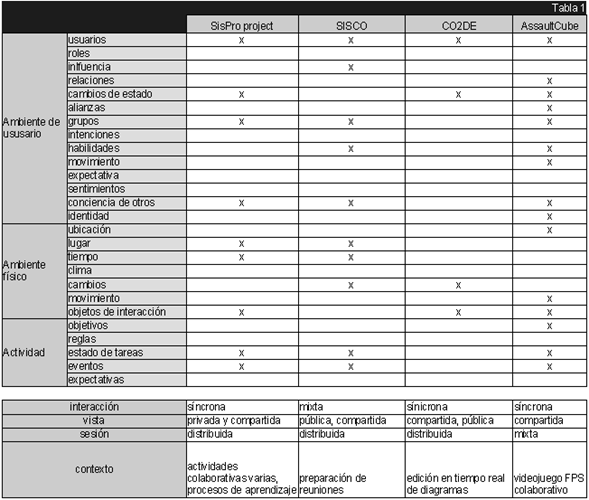
\includegraphics[scale=0.9]{groupware}
  \caption{Comparaci\'on de sistemas groupware}
  \label{cmp:gw}
\end{figure}

Como se puede observar en la figura \ref{cmp:gw} no todos los sistemas abarcan los mismos aspectos contextuales, cada uno tiene una arquitectura singular creada para satisfacer las necesidades del entorno para el que fueron creadas. 

En este trabajo se hace una propuesta de una arquitectura que pueda integrarse en cualquier tipo de sistema. Esta arquitectura tendr\'a soporte para el ambiente de aplicaciones ya que al ser el sistema groupware una entidad en el trabajo colaborativo, tiene que tener conciencia de s\'i misma y de otros sistemas que la rodean, incluyendo servicios, dispositivos, sensores, etc.

